% common part for every lection

\documentclass{beamer}

\usetheme{Warsaw}
\usefonttheme[onlylarge]{structurebold}
\setbeamerfont*{frametitle}{size=\normalsize,series=\bfseries}
\setbeamertemplate{navigation symbols}{}

\usepackage{pdfpages}
\usepackage{soul}
\usepackage{ucs}
\usepackage[utf8x]{inputenc}
\usepackage[TS1,T2A]{fontenc}
\usepackage[english,russian]{babel}
\usepackage{times}
\usepackage{listings}

\author[Author, Vlad Shakhov]{Влад 'mend0za' Шахов\\Linux \& Embedded Team Leader}

\institute[SaM Solutions]
{
  Linux \& Embedded Department
}

\date[Dec 2012]

\subject{Linux QA training}

\pgfdeclareimage[height=1.5cm]{sam-solutions-logo}{clipart/sam-solutions-elinux}

\logo{\pgfuseimage{sam-solutions-logo}}

\graphicspath{{./clipart/}}



\title[SaM Solutions. Linux QA Training]
{
  Занятие 2.\\
  Bourne Shell aka POSIX sh.
}

\begin{document}
\begin{frame}
  \titlepage
\end{frame}

\begin{frame}
  \frametitle{Что такое Unix shell?}
  
  \alert{Что такое Unix shell? (Назойливый повтор)}

  \begin{itemize}
    \item Обычная программа, запускающаяся после входа в систему
    \item Интерактивный командный интерпретатор
    \item Язык программирования
    \item Платформа интеграции (для утилит)
    \item Сотни разных реализаций (bash, ksh, zsh, tcsh, \ldots )
    \item Масса различных диалектов
  \end{itemize}

\end{frame}

\begin{frame}[fragile]
  \frametitle{Shell. Ключевые понятия - 1}
  \framesubtitle{Определения}

  \begin{itemize}
    \item \alert{Приглашение командной строки (CMD PROMPT)}: \pause 
      \begin{verbatim}
	$, #, user@host:~$
      \end{verbatim} \pause
    \item \alert{Команда}: \pause \newline \verb+whoami; top; exit+ \pause
    \item \alert{Параметр}: \pause \newline \verb+man bash; who am i+ \pause
    \item \alert{Ключ}: \pause \newline \verb+ls -a; ls -al; ls -al /tmp/+ 
  \end{itemize}
\end{frame}

\begin{frame}
  \frametitle{Shell. Ключевые понятия - 2}
  \framesubtitle{Картинка для закрепления}
    \hbox{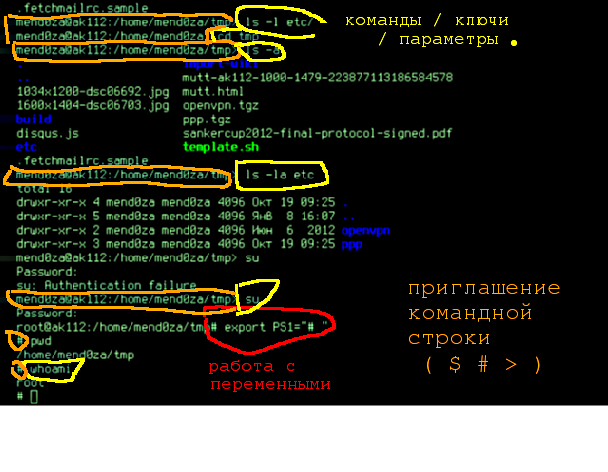
\includegraphics[height=7cm]{bash-input-screenshot}}
\end{frame}

\end{document}
